\section{Introduction}

\subsection{Motivation}

The Web is a rich source of information but is not a stable one, unfortunately. Indeed, one might read a controversial blog post, make a case against it to finally see its original content updated or removed with no way to prove what has been originally posted. This is only one of the many cases where having a proof that some online content was once available at some point would be a great help for users. We can think of journalists who could then cite online articles, or online victims who could prove they have been harassed, even if the actual content has been removed. The aim of this project is to propose a browser plugin that allows users to certify the content of some web pages at anytime.

\subsection{Context}

My work is in line with the decentralized system using "cothority" (collective authority), a framework to develop, analyze and deploy decentralized distributed protocols. This system is developed by the DEDIS laboratory. The entities running the protocol in a distributed way are called "cothority servers" or "conodes".

\subsubsection{Blockchain}

A blockchain can be seen as a linked-list with specific properties. It can also be a double linked-list. In this second case, we are talking about skipchains. Blockchains are constituted of blocks that contain digital pieces of information and can be perceived as a "distributed" database of records of all events that happened and  were shared among participating parties - each block being one of such event.
All network participants, which are conodes in our case, must agree on events that are added to the chain. This is achieved through the use of consensus algorithms - in this case, proof-of-consensus.

\subsubsection{Byzcoin}

I worked with "Byzcoin", which implements the distributed ledger called OmniLedger \cite{omniledger}. OmniLedger is a skipchain whose purpose is to preserve security under permissionless operations. Moreover, it is also designed to scale-out without compromising the security.

\subsubsection{Smart contracts}

In my project, I also have to implement a new smart contract. A smart contract is a digital protocol that guarantees the automatic execution of a contract when the agreed conditions are met. They allow agreements to be processed without the need for a third party to verify or enforce them. Moreover, they are traceable and irreversible.
In the context of this project, the smart contract will certify that the content of some web page existed at some time t. When such a contract is created to certify the content of a website, we call it an instance, and its corresponding instance ID will uniquely identify it.

\subsection{Goal}

This project consisted of, first, implementing a smart contract that would certify the content of a web page with the aid of a decentralized, proof-of-consensus, and blockchain-based ledger. Then, I also had to implement a browser plugin that would allow users to use this smart contract in an intuitive and easy way.
The plugin aims to provide a way for internet users to prove the existence of some content on a web page at some time.
Figure \ref{fa} shows how it works. When Alice is consulting the web page she wants to certify,  she can use the plugin ALINE on her laptop that will connects to the cothority and each node will get the content and if they reach a consensus, the smart contract will be spawned and its instance ID returned to Alice.


\begin{figure}[H]
    \centering
    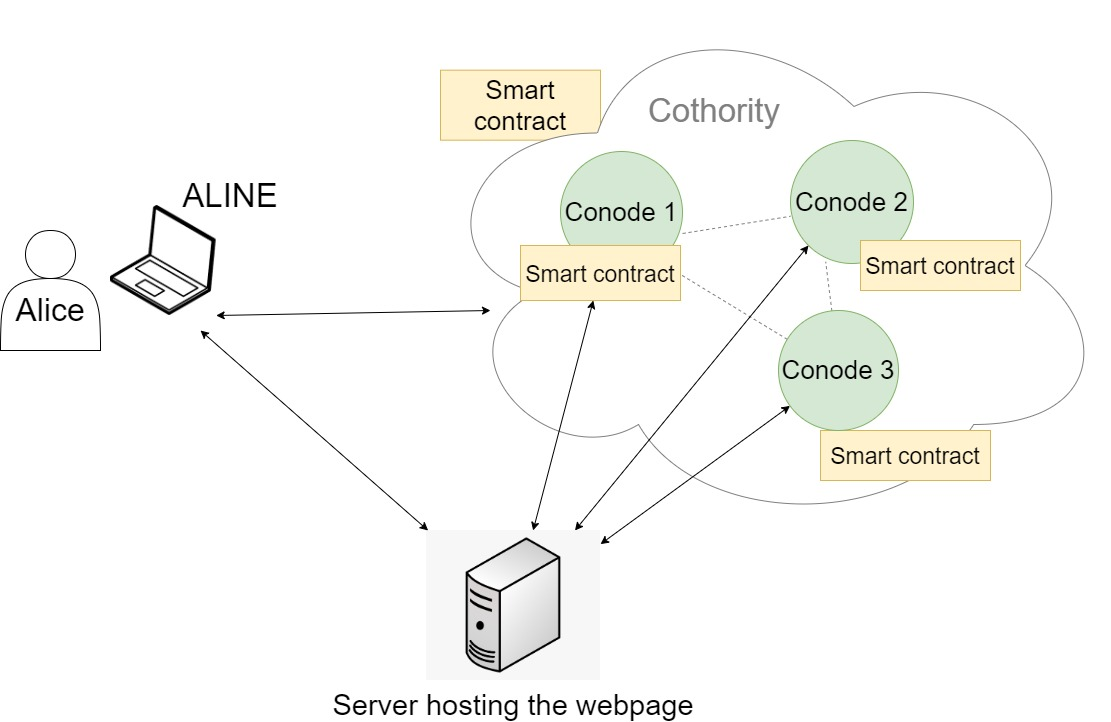
\includegraphics[width=1\linewidth]{images/Alice.jpg}
    \caption{ }
    \label{fa}
\end{figure}


